\documentclass[a4paper,11pt]{article}
\usepackage[utf8]{inputenc}
\usepackage[english]{babel}
\usepackage[T1]{fontenc}
\usepackage{amsfonts}
\usepackage{amsmath}
\usepackage{amssymb}
\usepackage{verbatim}
\usepackage{tikz}
\usepackage{graphicx}
\usepackage{color}
\usepackage{pgfpages}
\usepackage[final]{pdfpages}
\usepackage[square,sort]{natbib}
\date{15 Octobre 2015} 
\title{User Manual} 
\author{UF-yUML}

\begin{document}
\maketitle
\vskip 60pt
\section*{Introduction}
This document is given you some keys to use the UF-yUML project, and especially to deals with the syntax.
The UF-yUML project allows you to draw very easyly UML diagramm, and generate the associate java code, in an Object-Oriented way. \\ \\

\textbf{Installation :}

This project is based on yuml 0.1 (https://pypi.python.org/pypi/yuml). In order to use UF-yUML, you will need to install yuml 0.1 (github repository : https://github.com/wandernauta/yuml/).
Once you've install yuml 0.1, you only need to clone the UF-yUML in the same folder.\\

\textbf{Utilisation :}

First, you need to create a folder to your project.

Then, create in your project folder a class folder name "class". This folder will contains all the informations about your classes (attributes, methods), with one file for one class. Section \ref{module} shows you how to fill a class file with all its informations.

The next step is to build liaisons between your classes. Create one or more file in your folder project whose name begins by "liaisons". The section \ref{liaisons} shows you how to fill a liaisons file.

After running (see Section \ref{run} dealing with the run commands), UF-yUML will create a file diagramm.*** in your folder path with your project folder, and create a folder named "java" with your java code if needed (see Section \ref{java}).

\section{Run commands}
\label{run}
The typical run command is :
\begin{verbatim}
python uf-yuml.py -f folder/
\end{verbatim}
\textbf{Options :}

Only the -f is required

\begin{enumerate}
\item[-p] the name of your project folder
\item[-f] the output format: svg, png or pdf (default: png).
\item[-s] the UML output shape: scruffy, nofunky or plain (default: plain).
\item[-j] the java code generator: True or False (default False)
\item[-g] automatics getter and setter: True are False (default False).
\item[-m] displays the methods in the UML diagramm: True or False (default False).
\end{enumerate}

\section{Classes (or Interface, etc...)}
\label{module}
One class file is divided into three parts : the name, the attributs and the methods.

The following class file :
\begin{center}
\begin{verbatim}
Classe name

Attribut1
Attribut2

Method1
Method2
\end{verbatim}
\end{center}
will gave the following UML result :
\begin{center}
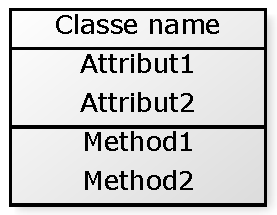
\includegraphics[width=4cm]{class}
\end{center}

\section{Liaisons}
\label{liaisons}
Each row of a liaisons file corresponf to a liaison. The format of a row is :
\begin{verbatim}
name_1,-,name_2
\end{verbatim}

name\_1 and name\_2 are the names of the two class you want to relie. - correspond to a simple line without arrow. You can change this string to change the shape of your line. Here are somes examples:

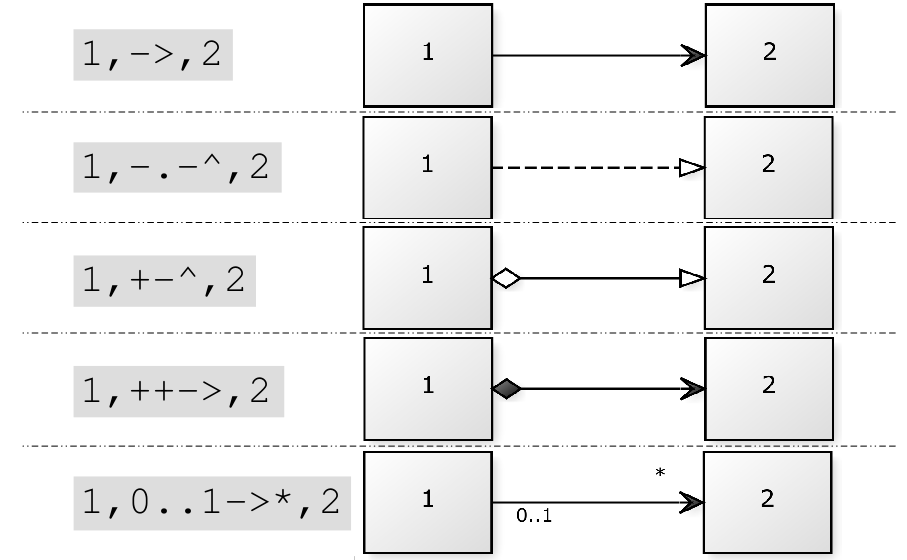
\includegraphics[width=13cm]{liaisons2}


You can also use space for your classes names, or use << for an interface:

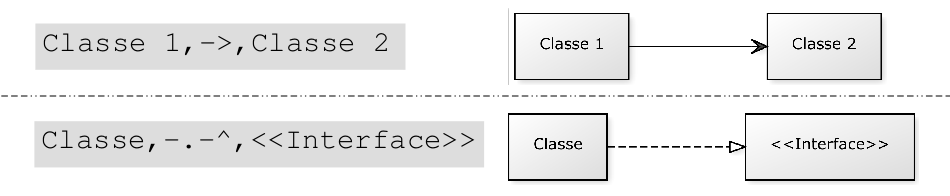
\includegraphics[width=13cm]{liaisons1}

\section*{Java generator}
\label{java}
If you want to generate java code, you have to respect some syntaxic rules about class files.
In particularly:

\begin{itemize}
\item Interfaces format must be <<name>>.
\item Interfaces implementations must be like $-.-^{\wedge}$
\item Classes heritage must be like $-^{\wedge}$
\item Attributs format must be like "name: type"
\item Methods format must be like "name(arguments): type"
\item Public attributs or methods must begin by "+ "
\item Private attributs or methods must begin by "- "
\end{itemize}

\end{document}